\begin{center}\section*{Abstract}\end{center}
\thispagestyle{empty}

This project looks at transforming a provided electrically powered go-kart into an autonomous vehicle capable of driving and navigation without human assistance. We have three main goals for this project. The first is to integrate a drive by wire system into the go-kart, so that it can be easily controlled by a laptop. The second is to develop a code that makes use of on-board sensors and the drive by wire system to execute a simple autonomous algorithm. This algorithm will follow a marker allowing the kart to automatically follow a person or vehicle. Finally while we wish to progress further and develop a program that will allow the kart to detect obstacles and navigate between GPS points we believe that we will not have sufficient time to make any significant progress towards this final goal. To date we have developed schematics and detailed plans for the drive by wire system. We have begun order parts and will begin putting together the systems in the next few weeks.

\vfill
  \begin{figure}[h]
    \centering
    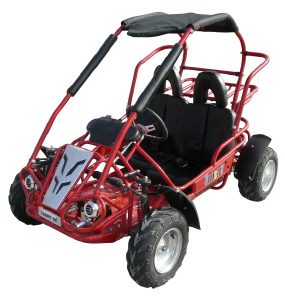
\includegraphics{../../Images/hh80h.jpg}
    \label{gokart}
  \end{figure}

% The abstract should be written assuming no other part of the report is read. A
% short statement about what your project is, what its goals are, progress made
% to date, and outlook for completing major project tasks is really what we’re
% looking for.

